\documentclass{beamer}

\input{settings.tex}


\title{Quadratically constrained quadratic programming, \\ Second-order cone programming}
\subtitle{Computational Intelligence, Lecture 9}
\author{by Sergei Savin}
\centering
\date{\mydate}



\begin{document}
\maketitle


\begin{frame}{Content}

\begin{itemize}
\item  Quadratic programming: recap
\item  Quadratically constrained quadratic programming
\begin{itemize}
    \item General form
    \item Domain
\end{itemize}
\item  Second-order cone programming
\begin{itemize}
    \item General form
    \item Special cases
    \item Friction cone
    \item Friction cone, solution
\end{itemize}
\item Homework
\end{itemize}

\end{frame}



\begin{frame}{Quadratic programming}
\framesubtitle{General form}
\begin{flushleft}

Remember the general form of a quadratic program:

%
\begin{equation}
\begin{aligned}
& \underset{\mathbf{x}}{\text{minimize}}
& & \mathbf{x}^\top \mathbf{H} \mathbf{x} + \mathbf{f}^\top\mathbf{x}, \\
& \text{subject to}
& & \begin{cases}
    \mathbf{A}\mathbf{x} \leq \mathbf{b}, \\
    \mathbf{F}\mathbf{x} = \mathbf{g}.
    \end{cases}
\end{aligned}
\end{equation}

where $\mathbf{H}$ is positive-definite and $\mathbf{A}\mathbf{x} \leq \mathbf{b}$ describe a convex region.
 
\end{flushleft}
\end{frame}




\begin{frame}{Quadratically constrained quadratic programming}
\framesubtitle{General form}
\begin{flushleft}

General form of a quadratically constrained quadratic program (QCQP) is given below:

%
\begin{equation}
\begin{aligned}
& \underset{\mathbf{x}}{\text{minimize}}
& & \mathbf{x}^\top \mathbf{P}_0 \mathbf{x} + \mathbf{q}_0^\top\mathbf{x}, \\
& \text{subject to}
& & \begin{cases}
    \mathbf{x}^\top \mathbf{P}_i \mathbf{x} + \mathbf{q}_i^\top\mathbf{x} + r_i \leq 0, \\
    \mathbf{F}\mathbf{x} = \mathbf{g}.
    \end{cases}
\end{aligned}
\end{equation}

where $\mathbf{P}_i$ are positive-definite.
 
\end{flushleft}
\end{frame}



\begin{frame}{Quadratically constrained quadratic programming}
\framesubtitle{Domain}
\begin{flushleft}

Domain of a QCQP without equality constraints and with no degenerate inequality constraints is an intersection of ellipses:

\begin{figure} [h!]
\begin{center}
\input{fig_1.tex}
\end{center} 
% \caption{AR 601 bipedal robot, Innopolis University}
\end{figure}
 
\end{flushleft}
\end{frame}



\begin{frame}{QCQP to QP and LP}
% \framesubtitle{General form}
\begin{flushleft}

Set $\mathbf{P}_i = \mathbf{0}$ and you get a QP.
%
\begin{equation}
\begin{aligned}
& \underset{\mathbf{x}}{\text{minimize}}
& & \mathbf{x}^\top \mathbf{P}_0 \mathbf{x} + \mathbf{q}_0^\top\mathbf{x}, \\
& \text{subject to}
& & \begin{cases}
    \begin{bmatrix} 
    \mathbf{q}_1^\top \\ ... \\ \mathbf{q}_n^\top
    \end{bmatrix} 
    \mathbf{x} \leq
    \begin{bmatrix} 
    r_1 \\ ... \\ r_n
    \end{bmatrix} \\
    \mathbf{F}\mathbf{x} = \mathbf{g}.
    \end{cases}
\end{aligned}
\end{equation}

Set $\mathbf{P}_0 = \mathbf{0}$ and you get an LP.

\end{flushleft}
\end{frame}




\begin{frame}{Second-order cone programming (SOCP)}
\framesubtitle{General form}
\begin{flushleft}


The general form of a Second-order cone program (SOCP) is:

%
\begin{equation}
\begin{aligned}
& \underset{\mathbf{x}}{\text{minimize}}
& & \mathbf{f}^\top\mathbf{x}, \\
& \text{subject to}
& & \begin{cases}
    ||\mathbf{A}_i\mathbf{x} + \mathbf{b}_i||_2 \leq 
     \mathbf{c}_i^\top \mathbf{x} + d_i, \\
    \mathbf{F}\mathbf{x} = \bo{g}.
    \end{cases}
\end{aligned}
\end{equation}

LP, QP and QCQP are subsets of SOCP.
 
\end{flushleft}
\end{frame}




\begin{frame}{SOC constraints, 1}
%	\framesubtitle{General form}
	\begin{flushleft}
		
		Consider the following SOC constraint:
		
		\begin{equation}
			\label{eq:SOC}
			||\mathbf{A}\mathbf{x} + \mathbf{b}||_2 \leq 
			\mathbf{c}^\top \mathbf{x} + d
		\end{equation}
		
		Let us consider a special case when $\mathbf{x} \in \R^n$, $\text{rank}\left(\begin{bmatrix}
			\mathbf{A} \\ \mathbf{c}^\top
		\end{bmatrix}\right) = n$. Then we can introduce the following substitution:
		
		\begin{equation}
			\xi = \begin{bmatrix}
				\mathbf{A} \\ \mathbf{c}^\top
			\end{bmatrix}
			\mathbf{x} + 
			\begin{bmatrix}
				\mathbf{b} \\ d
			\end{bmatrix}, 
		\ \ \ 
		\mathbf{I} = 
		\begin{bmatrix}
			\mathbf{E} \\ \mathbf{e}^\top
		\end{bmatrix}
		\end{equation}
%
where $\mathbf{I} \in\R^{n, n}$ is an identity matrix. Then constraint \eqref{eq:SOC} becomes:

		\begin{equation}
	||\mathbf{E}\xi||_2 \leq 
	\mathbf{e}^\top \xi
		\end{equation}
		
	\end{flushleft}
\end{frame}


\begin{frame}{SOC constraints, 2}
	%	\framesubtitle{General form}
	\begin{flushleft}
		
		Notice that $||\mathbf{E}\xi||_2 \leq 
		\mathbf{e}^\top \xi$ is equivalent to:
		
		\begin{equation}
			\sum\limits_{i=1}^{n-1}\xi_i^2 \leq \xi_n^2 
		\end{equation}
%	
	which is a standard form of a cone. A map back from $\xi$ to $\mathbf{x}$ is given as:
	
	\begin{equation}
		\mathbf{x} = \begin{bmatrix}
			\mathbf{A} \\ \mathbf{c}^\top
		\end{bmatrix}^{-1}
	\left(
		\xi - 
		\begin{bmatrix}
			\mathbf{b} \\ d
		\end{bmatrix}
	\right)
	\end{equation}
		
	\end{flushleft}
\end{frame}








\begin{frame}{Second-order cone programming}
\framesubtitle{Special cases}
\begin{flushleft}

We can write problem where our domain is a ball as SOCP:
%
\begin{equation}
\begin{aligned}
& \underset{\mathbf{x}}{\text{minimize}}
& & \mathbf{f}^\top\mathbf{x}, \\
& \text{subject to}
& & ||\mathbf{x}||_2 \leq d_i
\end{aligned}
\end{equation}

\bigskip

Same for ellipsoidal constraints:
%
\begin{equation}
\begin{aligned}
& \underset{\mathbf{x}}{\text{minimize}}
& & \mathbf{f}^\top\mathbf{x}, \\
& \text{subject to}
& & ||\mathbf{A}_i\mathbf{x}||_2 \leq d_i
\end{aligned}
\end{equation}
 
\end{flushleft}
\end{frame}




\begin{frame}{SOCP to QCQP}
\framesubtitle{Part 1}
\begin{flushleft}

Set $\mathbf{c}_i = 0$ and recognize that $||\mathbf{A}_i\mathbf{x} + \mathbf{b}_i||_2 \leq d_i$ is the same as $(\mathbf{A}_i\mathbf{x} + \mathbf{b}_i)^\top (\mathbf{A}_i\mathbf{x} + \mathbf{b}_i) \leq d_i^2$ (since the first implies that $d_i$ is non-negative).

\bigskip
%
\begin{equation}
\begin{aligned}
& \underset{\bo{x}}{\text{minimize}}
& & \bo{f}^\top\bo{x}, \\
& \text{subject to}
& & \begin{cases}
    \bo{x}^\top \bo{A}_i^\top \bo{A}_i \bo{x} + 
    2 \bo{b}_i^\top \bo{A}_i\bo{x} + 
    \bo{b}_i^\top \bo{b}_i  \leq d_i^2\\
    \bo{F}\bo{x} = \bo{g}.
    \end{cases}
\end{aligned}
\end{equation}

\end{flushleft}
\end{frame}




\begin{frame}{SOCP to QCQP}
\framesubtitle{Part 2}
\begin{flushleft}


Now to make the cost quadratic:
%
\begin{equation}
\begin{aligned}
& \underset{\bo{x}, t}{\text{minimize}}
& & t, \\
& \text{subject to}
& & \begin{cases}
    \bo{x}^\top \bo{A}_0^\top \bo{A}_0 \bo{x} + 
    2 \bo{b}_0^\top \bo{A}_0\bo{x} + 
    \bo{b}_0^\top \bo{b}_0  \leq t\\
    \bo{x}^\top \bo{A}_i^\top \bo{A}_i \bo{x} + 
    2 \bo{b}_i^\top \bo{A}_i\bo{x} + 
    \bo{b}_i^\top \bo{b}_i  \leq d_i^2\\
    \bo{F}\bo{x} = \bo{g}.
    \end{cases}
\end{aligned}
\end{equation}

Which is the same as:
%
\begin{equation}
\begin{aligned}
& \underset{\bo{x}}{\text{minimize}}
& & \mathbf{x}^\top \mathbf{H} \mathbf{x} + \mathbf{f}^\top\mathbf{x}, \\
& \text{subject to}
& & \begin{cases}
    \bo{x}^\top \bo{A}_i^\top \bo{A}_i \bo{x} + 
    2 \bo{b}_i^\top \bo{A}_i\bo{x} + 
    \bo{b}_i^\top \bo{b}_i  \leq d_i^2\\
    \bo{F}\bo{x} = \bo{g}.
    \end{cases}
\end{aligned}
\end{equation}

As long as $\bo{A}_0 = \sqrt{\bo{H}}$, and $\bo{b}_0 = 0.5 \bo{A}_0^{-1} \mathbf{f}$.

\end{flushleft}
\end{frame}




\begin{frame}{Friction cone}
\framesubtitle{Normal reaction force and friction}
\begin{flushleft}

\begin{figure}
    \centering
    

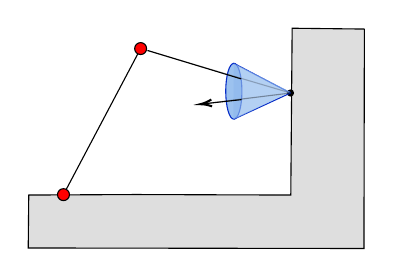
\begin{tikzpicture}[x=0.75pt,y=0.75pt,yscale=-0.5,xscale=0.5]
%uncomment if require: \path (0,300); %set diagram left start at 0, and has height of 300

%Straight Lines [id:da511009501867824] 
\draw    (150.25,190.35) -- (224.6,49.6) ;
%Shape: Polygon [id:ds12621320375323086] 
\draw  [fill={rgb, 255:red, 222; green, 222; blue, 222 }  ,fill opacity=1 ] (440.2,30.8) -- (370.6,30) -- (369.29,190.75) -- (219.79,190.25) -- (116.79,190.75) -- (116.29,241.75) -- (439.79,242.25) -- cycle ;
%Shape: Circle [id:dp8262097043760679] 
\draw  [fill={rgb, 255:red, 0; green, 0; blue, 0 }  ,fill opacity=1 ] (366.13,92.4) .. controls (366.13,90.81) and (367.41,89.53) .. (369,89.53) .. controls (370.59,89.53) and (371.88,90.81) .. (371.88,92.4) .. controls (371.88,93.99) and (370.59,95.28) .. (369,95.28) .. controls (367.41,95.28) and (366.13,93.99) .. (366.13,92.4) -- cycle ;
%Shape: Circle [id:dp2680036705913309] 
\draw  [fill={rgb, 255:red, 255; green, 0; blue, 0 }  ,fill opacity=1 ] (144.5,190.35) .. controls (144.5,187.17) and (147.07,184.6) .. (150.25,184.6) .. controls (153.43,184.6) and (156,187.17) .. (156,190.35) .. controls (156,193.53) and (153.43,196.1) .. (150.25,196.1) .. controls (147.07,196.1) and (144.5,193.53) .. (144.5,190.35) -- cycle ;
%Shape: Ellipse [id:dp3954723668349849] 
\draw  [color={rgb, 255:red, 0; green, 39; blue, 198 }  ,draw opacity=0.97 ][fill={rgb, 255:red, 156; green, 194; blue, 239 }  ,fill opacity=1 ] (306.6,90.7) .. controls (306.6,75.84) and (310.09,63.8) .. (314.4,63.8) .. controls (318.71,63.8) and (322.2,75.84) .. (322.2,90.7) .. controls (322.2,105.56) and (318.71,117.6) .. (314.4,117.6) .. controls (310.09,117.6) and (306.6,105.56) .. (306.6,90.7) -- cycle ;
%Straight Lines [id:da41806140316108764] 
\draw [color={rgb, 255:red, 0; green, 39; blue, 198 }  ,draw opacity=0.97 ][fill={rgb, 255:red, 156; green, 194; blue, 239 }  ,fill opacity=1 ]   (314.4,63.8) -- (369,92.4) ;
%Straight Lines [id:da8734911464392034] 
\draw [color={rgb, 255:red, 0; green, 39; blue, 198 }  ,draw opacity=0.97 ][fill={rgb, 255:red, 156; green, 194; blue, 239 }  ,fill opacity=1 ]   (314.4,117.6) -- (369,92.4) ;

%Flowchart: Merge [id:dp07751328773533905] 
\draw  [color={rgb, 255:red, 0; green, 0; blue, 0 }  ,draw opacity=0 ][fill={rgb, 255:red, 143; green, 185; blue, 237 }  ,fill opacity=0.68 ] (314.4,63.8) -- (313.88,118.01) -- (369.01,91.43) -- cycle ;
%Straight Lines [id:da8106680503102979] 
\draw [color={rgb, 255:red, 0; green, 0; blue, 0 }  ,draw opacity=0.24 ]   (224.6,49.6) -- (369,92.4) ;
%Straight Lines [id:da5735853405821096] 
\draw [color={rgb, 255:red, 0; green, 0; blue, 0 }  ,draw opacity=0.36 ]   (369,92.4) -- (282.2,103.2) ;
%Straight Lines [id:da788051954899972] 
\draw    (321.8,98.8) -- (284.19,102.98) ;
\draw [shift={(282.2,103.2)}, rotate = 353.65999999999997] [color={rgb, 255:red, 0; green, 0; blue, 0 }  ][line width=0.75]    (10.93,-3.29) .. controls (6.95,-1.4) and (3.31,-0.3) .. (0,0) .. controls (3.31,0.3) and (6.95,1.4) .. (10.93,3.29)   ;
%Straight Lines [id:da2615117595464225] 
\draw    (231.29,51.43) -- (321.4,78.8) ;
%Shape: Circle [id:dp33456176340238253] 
\draw  [fill={rgb, 255:red, 255; green, 0; blue, 0 }  ,fill opacity=1 ] (218.85,49.6) .. controls (218.85,46.42) and (221.42,43.85) .. (224.6,43.85) .. controls (227.78,43.85) and (230.35,46.42) .. (230.35,49.6) .. controls (230.35,52.78) and (227.78,55.35) .. (224.6,55.35) .. controls (221.42,55.35) and (218.85,52.78) .. (218.85,49.6) -- cycle ;




\end{tikzpicture}

    % \caption{}
    \label{fig:contact}
\end{figure}

Let $\bo{f}$ be total reaction force, $\bo{f}_n$ be its normal component (perpendicular to the surface locally), also known as normal reaction; and let $\bo{f}_{fr}$ be its tangential component (a vector lying in the tangent plane to the surface, constructed at the contact point), or friction force. Let $\mathbf{e}_n$ be a unit vector, normal to the surface at the point of contact.

\begin{equation}
    \bo{f} =  \bo{f}_n + \bo{f}_{fr}
\end{equation}

\end{flushleft}
\end{frame}



\begin{frame}{Second-order cone programming}
\framesubtitle{Friction cone}
\begin{flushleft}

Defining $\bo{E}_t = [\mathbf{e}_{t, 1}, \ \mathbf{e}_{t, 2}] = \mathcal{L}(\mathbf{e}_n)$ be an orthonormal basis in the tangential space to the surface, we can write:
%
\begin{align*}
\label{friction_cone}
    & \bo{f} = \mathbf{e}_n n + \bo{E}_t \bo{t} & \\
    & \bo{f}_n = \mathbf{e}_n n & \\
    & \bo{f}_{fr} = \bo{E}_t \bo{t} & \\
    & \bo{t} = [t_1, \ t_2]
\end{align*}
%
The friction cone conditions could be written in any of the following ways:
%
\begin{equation}
\label{friction_cone}
    \sqrt{t_1^2 + t_2^2} < \mu n
\end{equation}
%
\begin{equation}
    || \bo{E}_t^\top \mathbf{f} || \leq \mu \mathbf{e}_n^\top \mathbf{f}
\end{equation}
%
where $\mu$ is a friction coefficient.
 
\end{flushleft}
\end{frame}



\begin{frame}{Homework}
% \framesubtitle{Parameter estimation}
\begin{flushleft}

Implement a program that finds right-most point of an intersection of two ellipsoids; visualise the problem and the solution.

\end{flushleft}
\end{frame}




\begin{frame}
	\centerline{Lecture slides are available via Moodle.}
	\bigskip
	\centerline{You can help improve these slides at:}
	\centerline{
		\mygit
	}
	\bigskip
	
	\textcolor{black}{\qrcode[height=1.5in]{https://github.com/SergeiSa/Computational-Intelligence-Slides-Spring-2022}}
	\bigskip
	
	
	\centerline{Check Moodle for additional links, videos, textbook suggestions.}
\end{frame}



\end{document}
